%!LW recipe=latexmk (xelatex)
\documentclass[14pt, a4paper, fleqn, titlepage]{extarticle}
\usepackage{styles/mystyle}
\usepackage{tocloft}
% \usepackage{styles/titlepage}
% \usepackage{styles/titlepagepractice}

\renewcommand{\thesection}{ГЛАВА~\arabic{section}}
\renewcommand{\thesubsection}{\arabic{section}.\arabic{subsection}} 
\renewcommand{\thesubsubsection}{\thesubsection.\arabic{subsubsection}}
\renewcommand{\thefigure}{\arabic{section}.\arabic{figure}}
\addto\captionsrussian{\renewcommand{\contentsname}{Оглавление}}
\setdefaultlanguage{russian}
\XeTeXlinebreaklocale "ru"
\XeTeXlinebreakskip = 0pt plus 1pt
\sloppy

\begin{document}
    \everymath{\displaystyle}

    
    
\includepdf[pages=1-2, fitpaper=true]{pictures/VKR_titlepage.pdf}
    \pagebreak

    \setcounter{page}{2}

    % \includepdf[pages=1-2, fitpaper=true]{pictures/zadanie.pdf}
    % \pagebreak

    %!LW recipe=latexmk (xelatex)
\section*{АННОТАЦИЯ}\addcontentsline{toc}{section}{АННОТАЦИЯ}

Выпускная квалификационная работа выполняет перенос и адаптацию логики сетевого прототипа RTS-игры с голосовым управлением с игрового движка Citrus, 
остававшегося на ранней стадии разработки и обладавшего ограниченной структурой, на кроссплатформенный Godot Engine с использованием C\#. 
Проведён сравнительный анализ игровых движков и голосовых технологий, обоснован выбор Godot, локальной ASR-библиотеки Vosk.CSharp и 
.NET SpeechSynthesizer. Реализованы ключевые модули: клиент-серверное взаимодействие, HUD, gRPC-обработка голосовых 
команд и серверная логика боёв. Результаты подтверждают повышение архитектурной гибкости, производительности и кроссплатформенности прототипа.
\section*{ABSTRACT}

This thesis ported and adapted the logic of a networked RTS game prototype with voice control from the Citrus game engine — then at an early development 
stage with limited tooling — to the cross-platform Godot Engine using C\#. A comparative analysis of game engines and voice technologies informed the
choice of Godot, the Vosk.CSharp ASR library, and the .NET SpeechSynthesizer. Core modules were implemented: client-server communication, 
HUD, gRPC-based voice command processing, and server-side battle logic. The results demonstrate improved architectural 
flexibility, performance, and cross-platform support.
    \pagebreak


    \tableofcontents
    \thispagestyle{fancy}
    \pagebreak

    %Убрать в приложение???
    % !TEX root =..\main.tex
\section*{ТЕРМИНЫ, ОПРЕДЕЛЕНИЯ И СОКРАЩЕНИЯ}\addcontentsline{toc}{section}{ТЕРМИНЫ, ОПРЕДЕЛЕНИЯ И СОКРАЩЕНИЯ}
В настоящей письменной работе применены следующие термины с
соответствующими определениями.

\textbf{Игровой движок} -- программная платформа, обеспечивающая отрисовку графики, обработку ввода, физику и другие базовые подсистемы для создания игр.

\textbf{Библиотека} -- набор готовых функций, классов и ресурсов, предназначенных для повторного использования в разных проектах.

\textbf{RTS} -- жанр стратегии в реальном времени, в котором игроки одновременно управляют базой, ресурсами и юнитами.

\textbf{Туман войны} -- механизм скрытия частей карты, недоступных прямому обзору игрока, обычно представленный затемнением или неразличимой текстурой.

\textbf{Юнит} -- игровой объект (единица), управляемый игроком или ИИ, например боевая единица в стратегии.

\textbf{ASR} -- система автоматического распознавания речи, преобразующая аудиосигнал в текст.

\textbf{TTS} -- система синтеза речи, генерирующая звуковую дорожку на основе текстовых данных.

\textbf{SDK} -- комплект средств разработки, включающий библиотеки, документацию и инструменты для создания ПО.

\textbf{HUD} -- интерфейс на экране (англ. Heads-Up Display), отображающий важные игровые параметры: здоровье, ресурсы, миникарту и т. п.

\textbf{gRPC} -- фреймворк для высокопроизводительного удалённого вызова процедур по протоколу HTTP/2.

\textbf{UDP} -- протокол пользовательских датаграмм без установления соединения и гарантии доставки, обеспечивающий низкую задержку.

\textbf{Клиент} -- компонент сети или приложения, отправляющий запросы серверу и получающий от него данные.

\textbf{Сервер} -- компонент сети или приложения, обрабатывающий запросы клиентов, хранящий данные и управляющий логикой.

\textbf{Кроссплатформенность} -- способность программного продукта работать на разных ОС и устройствах без существенных изменений кода.

\textbf{Сцена} -- в Godot структурированный набор узлов, сохраняемый в файле и инстанцируемый как единый объект.

\textbf{Узел} -- базовый строительный блок сцены в Godot, обладающий свойствами, методами и способностью быть частью иерархии.

\textbf{«горячая» перезагрузка} -- возможность обновить код или ресурсы приложения во время его выполнения без перезапуска.

\textbf{Тайл} -- графический элемент карты, организованный в сетку для построения игрового уровня.

\textbf{Ассет} -- ресурс проекта (спрайт, звук, шейдер и т. п.), импортируемый и используемый движком.

\textbf{Спрайт} -- растровое изображение, применяемое как игровой объект или элемент интерфейса.

\textbf{Текстура} -- графический ресурс, налагаемый на объекты сцены для их визуализации.

\textbf{Пакет} -- блок данных, передаваемый по сети между узлами приложения.

\textbf{Шейдер} -- программа для графического процессора, отвечающая за расчёт визуальных эффектов.

\textbf{P2P} -- архитектура «равный-равному», где узлы сети обмениваются данными напрямую без центрального сервера.

\textbf{Клиент-серверная архитектура} -- модель взаимодействия, где клиенты отправляют запросы центральному серверу, а он отвечает и управляет состоянием.

\textbf{WER} -- метрика ошибок распознавания речи (Word Error Rate), процент отличий между эталонным и распознанным текстом.

\textbf{CPU} -- центральный процессор, основной вычислительный блок компьютера.

\textbf{GPU} -- графический процессор, специализированный блок для вычислений, связанных с визуализацией и шейдерами.

\textbf{HTTPS} -- протокол защищённой передачи гипертекста поверх TLS/SSL на базе HTTP.

\textbf{End-to-End} -- задержка или процесс, охватывающий весь путь данных от отправителя до конечного получателя без промежуточных буферов.

\textbf{MVP} -- минимально жизнеспособный продукт, версия проекта с минимальным набором функций для проверки идеи.

\textbf{Z-индекс} -- параметр порядка отрисовки объектов, определяющий, какие элементы отображаются поверх других.

\textbf{Плагин} -- модуль или расширение для программы или движка, добавляющее новую функциональность без внесения изменений в её ядро.

\textbf{Рендеринг} -- процесс вычисления и вывода на экран визуального представления сцены или графики, включающий расчёт освещения, текстур и шейдеров.

\textbf{Singleton} -- порождающий шаблон проектирования, гарантирующий создание единственного экземпляра класса и обеспечивающий к нему глобальный доступ.
    \pagebreak

    % !TEX root =..\main.tex
\section*{ВВЕДЕНИЕ}\addcontentsline{toc}{section}{ВВЕДЕНИЕ}
    В последние годы в игровой индустрии наблюдается устойчивый рост интереса к естественно-речевым интерфейсам, которые делают взаимодействие 
    пользователя с виртуальным миром более интуитивным и доступным. Особенно перспективно применение голосового управления в жанре стратегии 
    реального времени (RTS): высокие темпы игры, многопользовательский режим и сложный микроменеджмент требуют от игрока быстрого и удобного 
    способа отдачи команд. Одновременно растут требования к кроссплатформенности и расширяемости игровых проектов, чему традиционные 
    узкоспециализированные движки зачастую не отвечают.

    Выпускная квалификационная работа посвящена разработке сетевой RTS-игры на языке C\# с интегрированным голосовым интерфейсом. В качестве основы 
    выбран свободный и кроссплатформенный движок Godot Engine, чья модульная архитектура и поддержка Mono позволяют унаследовать большую часть 
    логики существующего клиента на Citrus Engine, одновременно решив его фундаментальные ограничения, о которых пойдет речь в дальнейшем.

    Научная новизна исследования заключается в комплексной интеграции системы автоматического распознавания речи (ASR) и синтеза речи (TTS) в 
    многопользовательскую RTS-игру, построенной на Godot, а практическая значимость -- в создании масштабируемой архитектуры, пригодной для учебных и 
    демонстрационных целей, а впоследствии — для коммерческих проектов.

    Работа состоит из трёх глав. В первой главе <<Постановка задачи>> обоснованы актуальность темы, сформулированы цель и задачи 
    работы, приведён обзор исходного клиента и содержится обоснование выбора Godot. Вторая глава <<Теоретический анализ>> 
    содержит сравнительный обзор игровых движков, сетевых архитектур и ASR/TTS-решений. 
    Третья глава <<Разработка проекта>> описывает практическую реализацию клиент-серверной RTS-игры с голосовым управлением: 
    настройку окружения, перенос логики на новый движок, дополнение серверной логики. 
    В заключении приведены основные результаты и направления дальнейшего развития.
    \pagebreak

    
    % !TEX root =..\main.tex
\section{ПОСТАНОВКА ЗАДАЧИ}

    \subsection{Актуальность} 
    Жанр RTS продолжает занимать важное место в индустрии, предлагая игрокам сложные сценарии управления и координации большого числа юнитов. Традиционные средства управления (мышь и клавиатура) обеспечивают высокую точность, но требуют большой скорости и точности ввода игровых команд. Внедрение голосовых команд способно упростить управление, повысить скорость отдачи приказов и сделать игру более доступной для пользователей с особыми потребностями.

    Одновременно индустрия предъявляет всё более строгие требования к кроссплатформенности проектов и гибкости их архитектуры. Закрытые или узко ориентированные игровые движки ограничены поддержкой платформ и набором встроенных инструментов, что существенно тормозит развитие и масштабирование игры.

    В рамках курсовой работы был создан рабочий прототип сетевой RTS-игры на базе Citrus Engine с интегрированными модулями автоматического распознавания речи и синтеза речи. Однако, по мере расширения функционала выявились фундаментальные ограничения этой платформы.

    \subsection{Цель работы}
    Цель настоящей работы -- разработать и реализовать прототип сетевой RTS-игры на языке C\# с голосовым управлением, обеспечивающий:
    \begin{itemize}
        \item Устойчивое многопользовательское взаимодействие;
        \item Интеграцию локального ASR-модуля для распознавания голосовых команд;
        \item Модуль TTS-синтеза для обратной голосовой связи;
        \item Кроссплатформенный клиент на базе Godot Engine.
    \end{itemize}


    \subsection{Задачи}
    Для достижения поставленной цели необходимо решить следующие задачи:
    \begin{itemize}
    \item Провести анализ исходного прототипа на Citrus Engine, выявить его технические и организационные ограничения;
    \item Сформулировать требования к новому движку и обосновать выбор Godot;
    \item Адаптировать и перенести логику игрового цикла и сетевого взаимодействия на Godot + C\#;
    \item Реализовать клиентскую логику приёма голосовых команд, отрисовки игрового поля и воспроизведения аудиоответа.
    \end{itemize}

    \subsection{Недостатки исходного прототипа и обоснование перехода на Godot}
    Рабочий прототип на Citrus Engine включал клиент-серверную архитектуру, обработку пользовательского ввода, обмен игровым состоянием по протоколу UDP, а также интеграцию ASR и TTS через выделенные модули. При всём этом были выявлены следующие ограничения:
    \begin{itemize}
    \item Отсутствие кроссплатформенности, отсутствие экспорта в macOS, Linux и на мобильные устройства;
    \item Фрагментарная и неполная документация, слабая поддержка сообщества;
    \item Необходимость самостоятельной реализации многих низкоуровневых подсистем;
    \item Громоздкая структура проекта, препятствующая быстрой навигации и автоматизации сборки.
    \end{itemize}

    Для устранения этих недостатков выбран Godot Engine, обладающий:
    \begin{itemize}
    \item Полноценной кроссплатформенной поддержкой (Windows, Linux, macOS, iOS, Android, Web);
    \item Развитой системой сцен и узлов, позволяющей строить игровую логику модульно;
    \item Встроенной поддержкой C\# (Mono), упрощающей перенос существующего кода;
    \item Активным сообществом и большим количеством готовых аддонов в Asset Library;
    \item Возможностью <<горячей>> перезагрузки скриптов и гибкой настройкой проекта.
    \end{itemize}

    Переход на Godot обеспечивает сосредоточение основных усилий на развитии геймплейных механик и голосового интерфейса без отвлечения на реализацию базовых движковых подсистем.
    \pagebreak

    % !TEX root =..\main.tex
\section{ТЕОРЕТИЧЕСКИЙ АНАЛИЗ}

    \subsection{Анализ существующего прототипа на движке Citrus}

        В ходе курсовой работы был создан прототип двухмерной игры на движке Citrus Engine. Задачи прототипа включали: отображение анимации персонажа, 
        обработку пользовательского ввода, взаимодействие с сервером и отрисовку обновленного игрового состояния, обработку голосового потока и преобразование его в текст,
        а также генерацию голосового ответа для игрока. Игровой мир состоял из тайловых карт, загружаемых из текстовых файлов и набора спрайтов для визуализации окружающей среды и объектов.
        
        \subsubsection{Архитектура прототипа}

        В основе прототипа лежит клиент-серверная архитектура с выделенным модулем распознавания команд, модулем распознавания речи (ASR) и модулем синтеза речи (TTS). 
        Все компоненты взаимодействуют в рамках игрового цикла, обеспечивая прием голосовых команд от пользователя, их интерпретацию в игровые действия, 
        обновление состояния и обратную отдачу в виде визуального и звукового ответа. Основные блоки системы:

        \textbf{Клиентская часть}
        
        Отвечает за сбор голосового ввода от пользователя, передачу аудиопотока на сервер, десериализацию и отображение обновлённого игрового состояния. 
        После получения от сервера готовых данных клиент одновременно рендерит игровые объекты и воспроизводит аудиоответ.

        \textbf{Основной серверный процесс}
        
        Вся серверная часть контролируется основным процессом. При его запуске, в отдельном потоке инициализируются все модули проекта, а также
        в консоль выводится детальная информация о состоянии модулей с помощью библиотеки Terminal.Gui.
        \begin{lstlisting}[caption=Инициализация модулей]
var gameLoopThread = new Thread(GameLoop);
var networkThread = new Thread(NetworkLoop);
var broadcastThread = new Thread(BroadcastLoop);
var consoleThread = new Thread(ConsoleLoop);
var voiceEmitterThread = new Thread(VoiceEmitterLoop);
var voiceRecognitionTask = new Task(VoiceRecognitionLoop);
        \end{lstlisting}

        \textbf{Модуль распознавания команд}
        
        Принимает непрерывный аудиопоток от клиента, отправляет его на обработку в модуль ASR, 
        получает распознанный текст, затем преобразует его в формализованную игровую команду и передаёт на сервер.
        Список возможных команд продемонстрирован в таблице в \textbf{приложении Г}.

        \textbf{Модуль игровой логики}

        Получив игровую команду, сервер обновляет игровое состояние (положение юнитов, их здоровье и т.д.) и формирует один или 
        несколько объектов TaskResult, описывающих результаты действия (перемещение юнита, изменение ресурсов, возникновение событий и т. д.).
        Эти объекты передаются в очередь модуля TTS для дальнейшего синтеза аудиоответа. Одновременно с этим обновленное игровое состояние
        сериализуется, затем посредством библиотеки LiteNetLib и сетевого протокола UDP передается на клиент.

        \textbf{Модуль Text-to-Speech}
        
        Извлекает объект TaskResult из очереди и на его основе с помощью алгоритма синтеза речи генерирует аудиопоток с голосовым сообщением игр
        отправляет его на клиент по протоколу gRPC.

        \textbf{Канал возврата данных}
        
        Игра и модуль TTS завершают такт независимо: сервер отправляет клиенту обновлённое состояние, а TTS -- аудиопоток ответа. 
        Клиент обрабатывает оба результата <<по приходу>>, синхронно обновляя интерфейс и воспроизводя голосовое сообщение.
        

        \begin{figure}[H]
            \centering
            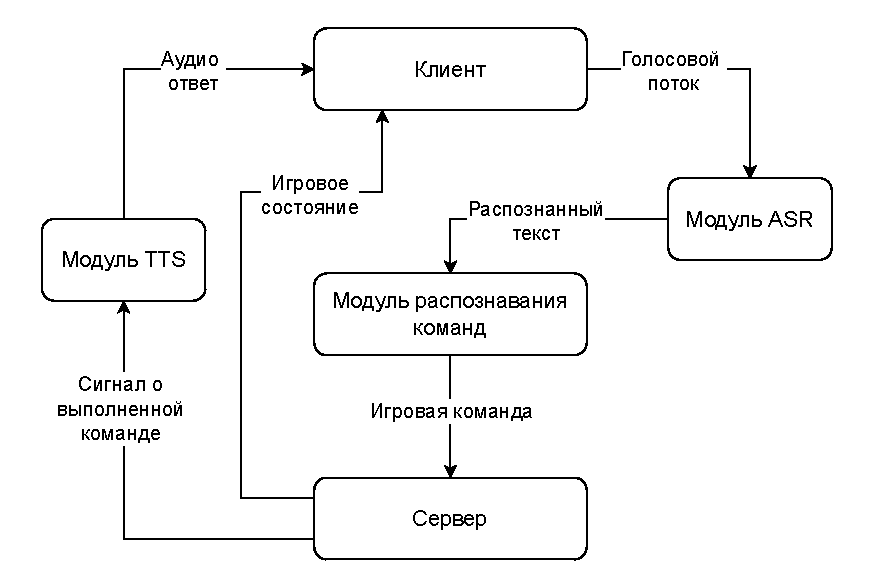
\includegraphics[scale=1]{pictures/architecture_scheme.pdf}
            \caption{Блок-схема архитектуры}\label{ris1.1}
        \end{figure}

        Такая архитектура (рисунок \ref{ris1.1}) позволяет гибко масштабировать голосовой интерфейс и логику игры, развивая каждый модуль отдельно: оптимизировать ASR-движок, улучшать логику генерации 
        TaskResult или внедрять новые голоса в TTS, не затрагивая остальные компоненты.

        \subsubsection{Игровой цикл}

        Игровой цикл прототипа можно свести к следующим этапам:

        \begin{itemize}
            \item пользователь на клиенте произносит голосовую команду;
            \item клиент шлёт аудиопоток на сервер, где модуль распознавания команд совместно с языковой моделью преобразует звук в текст и переводит его в формальную игровую команду;
            \item серверный игровой движок принимает команду, изменяет состояние и создаёт объекты TaskResult;
            \item тaskResult передаётся в модуль TTS, который синтезирует аудиоответ; одновременно обновлённое игровое состояние возвращается клиенту как отдельный пакет;
            \item клиентская часть отображает новый кадр игры и воспроизводит полученный голосовой ответ.
        \end{itemize}

        
        \subsubsection{Технические и организационные проблемы Citrus}

        В процессе разработки прототипа на Citrus стало ясно, что дальнейшее расширение проекта на этой платформе встретит серьёзные затруднения: сама экосистема 
        движка жёстко завязана на Windows, что исключает возможность экспорта приложения под Linux, macOS или мобильные устройства, а попытки 
        обойти это ограничение требуют непропорционально больших усилий и рисков несоответствия требованиям целевых платформ. Кроме того, официальная документация сводится 
        лишь к перечню классов и методов без каких-либо практических рекомендаций по построению архитектуры или описания сложных сценариев работы, поэтому разработчикам 
        приходится изучать движок эмпирическим путем, додумывая что делает тот или иной метод. Внутренняя организация движка избыточно детализирована и сильно загромождена кодом: 
        вместо того чтобы предоставить разработчику готовые, высокоуровневые абстракции для ввода-вывода, анимации и рендеринга, Citrus вынуждает 
        разбираться с низкоуровневыми реализациями и вручную настраивать связи между модулями. При этом отсутствуют 
        специализированные библиотеки или готовые плагины, которые могли бы взять на себя обработку ввода с контроллеров и клавиатуры, проигрывание сложных анимационных 
        последовательностей или оптимизированный отрисовочный конвейер, поэтому любую подобную функциональность приходится реализовывать самостоятельно поверх уже громоздкой, 
        неинтуитивной структуры движка. Постоянная необходимость вручную синхронизировать многочисленные файлы и конфигурации усложняет 
        сопровождение кода и практически исключает автоматизированный рефакторинг, а отсутствие активного сообщества, форумов, учебных курсов и открытых примеров практически 
        обесценивает любые усилия по поиску готовых решений или обмену опытом: каждый новый вопрос превращается в многодневный эксперимент, что полностью нивелирует преимущество 
        быстрой прототипизации.

        Все эти факторы делают дальнейшую разработку крупного или коммерчески значимого проекта на Citrus нецелесообразной. Для обеспечения кроссплатформенности, простоты поддержки 
        и быстрой интеграции необходимых модулей требуется смена движка.

    \subsection{Сравнительный анализ технологий}

        \subsubsection{Игровые движки}

        \textbf{Критерии выбора нового движка}

        При выборе альтернативного движка учитывались следующие критерии:
        \begin{itemize}
            \item поддержка языка программирования C\# (Поскольку существенная часть кода прототипа была написана именно на этом языке);
            \item кроссплатформенность (Windows, Linux, мобильные платформы);
            \item наличие и полнота документации, обучающих материалов, примеров;
            \item развитое сообщество и экосистема (Библиотека ассетов, плагины, расширения);
            \item простая и гибкая архитектура проектов (удобная структура сцен/сценариев, минимальная настройка конфигурационных файлов).
        \end{itemize}


        \textbf{Сравнение движков}

        \textbf{Citrus}

        Citrus -- игровой движок российской компании Game Forest, предназначенный для разработки 2D игр, 
        разрабатывающийся для внутреннего пользования, однако, также присутствует публичная версия. Поскольку он находится на ранних этапах разработки, 
        у него отсутствуют какие-либо справочные материалы, помимо плохо составленной документации. Также присутствует редактор сцен, который никак не 
        задокументирован, а его нагроможденность делает его практически бесполезным. Несмотря на это, он все же пригоден для создания игр, 
        но для разработчика, не имеющего отношения к этой компании, это будет весьма затруднительно. Вместе с движком предоставляются примеры готовых проектов 
        в жанре "платформер" и "3 в ряд" для ознакомления с его функционалом, однако, этого недостаточно для комфортной разработки RTS.

        \textbf{Unity}

        Unity давно зарекомендовал себя эталоном кроссплатформенной разработки: редактор доступен на Windows и macOS, экспорт проектов поддерживается на все актуальные настольные 
        операционные системы, iOS, Android и даже игровые консоли. Официальная документация Unity включает полные справочники API, пошаговые руководства, 
        обучающие видео и обширную базу примеров, что позволяет быстро освоиться как начинающим, так и опытным разработчикам. Развитое сообщество вокруг Unity гарантирует 
        наличие тысяч готовых плагинов и ассетов в Asset Store, регулярные обновления движка и ответы на наиболее частые вопросы на форумах и в тематических чатах. Архитектура проектов 
        в Unity строится вокруг концепции сцен и префабов (Prefabs): сцены организуются в упорядоченную и понятную иерархию игровых объектов, а конфигурационные файлы сведены к минимуму, 
        поскольку большая часть настроек хранится в самих префабах. Наконец, поддержка языка C\# является одной из сильных сторон Unity: весь пользовательский код пишется 
        именно на нём, что позволяет без портирования переиспользовать значительную часть логики из прототипа.
        
        \textbf{Unreal Engine}

        Unreal Engine демонстрирует хорошую кроссплатформенность на уровне экспорта -- проекты могут быть собраны под Windows, macOS, Linux, Web через Pixel Streaming, а также на 
        мобильные платформы и консоли. Документация Unreal отличается глубиной технических объяснений, однако основной упор сделан на C++ и визуальные скрипты Blueprint. 
        Сообщество Unreal велико, имеет собственный магазин ассетов и множество учебных курсов, но в сфере 2D-игр движок нередко воспринимают как <<тяжёлый>> и избыточный. 
        Архитектура проектов в UE сложнее: уровни, акторы, компоненты и классы C++ формируют мощную, но громоздкую структуру, требующую детального понимания внутренней логики движка. 
        Что касается C\#, официальной интеграции нет -- подобные возможности реализуются лишь через сторонние плагины и зачастую сопровождаются высокой затратой времени на настройку.
        
        \textbf{Godot}

        Godot представляет собой полностью свободный движок с редактором на Windows, Linux и macOS и универсальным экспортом под все популярные платформы, включая Web и мобильные ОС. 
        Документация Godot охватывает как справочник API, так и пошаговые гайды по разработке, а активное и быстро растущее сообщество регулярно публикует готовые демо-проекты и видеоуроки. 
        Встроенная Asset Library постепенно наполняется шаблонами и расширениями, хотя пока не достигает масштабности Unity Asset Store, но для 2D-игр базового набора достаточно.
        Проектная архитектура Godot основана на лёгкой и гибкой системе сцен и узлов: вместо многочисленных конфигураций создаются сцены, вложенные в другие сцены, и настраиваются связи 
        прямо в визуальном редакторе. Это позволяет быстро прототипировать и при этом легко масштабировать проект. Начиная с версии 3.x, Godot имеет полноценную поддержку C\# под управлением 
        Mono: код на C\# компилируется и выполняется наряду с GDScript, что облегчает перенос и развитие написанной ранее логики.

        \begin{table}[ht]
            \caption{Сравнение игровых движков}
            \centering
            \renewcommand{\arraystretch}{1.2}
            \renewcommand{\tablename}{Табл.}
            \begin{tabularx}{\textwidth}{|X|X|X|X|X|X|}
            \hline
            &\textbf{Поддержка C\#} & \textbf{Кросспла-тформенн-ость} & \textbf{Подробная документация} & \textbf{Размер сообщества} & \textbf{Простота освоения} \\
            \hline
            Citrus&Да&Нет&Нет& Нулевой&Тяжело\\
            \hline
            Unity&Да&Да&Да& Большой&Умеренно\\
            \hline
            Unreal&Нет&Да&Да&Большой&Очень тяжело\\
            \hline
            Godot&\textbf{Да}&Да&\textbf{Да}&Средний&\textbf{Легко}\\
            \hline
            \end{tabularx}
        \end{table}

        При сравнительной оценке по пяти ключевым критериям Unity и Godot отвечают всем требованиям: Unity выигрывает за счёт зрелости экосистемы и количества готовых решений, 
        Godot привлекает открытостью, лёгкостью проекта и достаточной поддержкой C\#. Unreal Engine, хотя и силён в 3D-разработке, не оптимален для C\#-ориентированной 2D-игры. 
        Учитывая баланс между простотой использования, быстрой кроссплатформенной сборкой, обилием документации и непосредственной поддержкой C\#, окончательным выбором стал Godot Engine.

        С переходом на Godot открывается целый набор средств для быстрой и гибкой доработки геймплея и интерфейса. Его система сцен и узлов позволяет 
        создавать многослойный HUD: Control-узлы и CanvasLayer и Control легко организуют главное меню, окно управления юнитами и всплывающие подсказки, 
        а встроенные Theme-ресурсы (StyleBox, Font) обеспечивают единый стиль и адаптивную вёрстку под разные разрешения экрана. Во-вторых, визуальный конвейер Godot 
        поддерживает 2D-шейдеры, благодаря чему <<туман войны>> можно реализовать прямо на GPU.

        Кроме того, сцены-шаблоны облегчают добавление новых игровых объектов и элементов пользовательского интерфейса: через наследование или композицию можно разграничить общие параметры 
        и уникальные скрипты поведения. Полноценная поддержка C\# и «горячая» перезагрузка скриптов (hot reload) сокращают время отладки: изменения в коде вступают в силу мгновенно, 
        без перезапуска игрового клиента, а кроссплатформенный экспорт (Windows, Linux, macOS, Android, iOS) позволяет сразу проверять поведение и производительность на любых целевых устройствах.

        Благодаря таким возможностям внедрение классических RTS-элементов станет удобным и оперативным: новые игровые объекты будут конфигурироваться визуально, а программная логика 
        останется сосредоточенной в читаемом и легко поддерживаемом коде. Вместо ручного переписывания низкоуровневых компонентов, появится возможность сфокусироваться на дизайне 
        баланса, сценариях развития игроков и качественном тестировании механик, что значительно ускорит трансформацию прототипа в полнофункциональную стратегию.

        \subsubsection{Сетевые архитектуры}

        В контексте разработки многопользовательских сетевых игр обычно применяют один из трех основных подходов: peer-to-peer, клиент-серверную архитектуру и гибридные решения. Ниже приведет краткий 
        обзор их сильных и слабых сторон:

        \textbf{Peer-to-Peer (P2P)}

        В P2P-сети каждый игрок напрямую обменивается сообщениями с остальными участниками. Такой подход позволяет избавиться от необходимости разработки серверной части 
        и минимизировать задержки при передаче команд, поскольку обмен пакетов происходит напрямую между игроками, однако для RTS-игр это требует строгой детерминированности игрового 
        движка (чтобы все клиенты, получив одни и те же команды, гарантированно пришли к одному и тому же состоянию мира) и сложной системы синхронизации (lockstep). Кроме того, 
        P2P-сети плохо масштабируются при большом числе участников и уязвимы к читерским вмешательствам. Дополнительно от клиента потребуются вычислительные мощности, чтобы распознавать текст
        из аудиопотока и синтезировать аудиоответ.
        
        \textbf{Клиент-серверная}

        Все действия игроков проходят через единый сервер, который проверяет валидность команд, обновляет состояние мира и рассылает клиентам результат. 
        Такой подход исключает необходимость в детерминированном движке, упрощает борьбу с читерством и централизует логику синхронизации. Сервер, обрабатывая запросы на управление 
        (в том числе текстовые команды из ASR), может дополнительно валидировать их через синтаксический разбор, фильтровать «спам» голосовых запросов и шифровать трафик. Выбор 
        клиент-серверной архитектуры для сетевой RTS обоснован следующими факторами. Во-первых, голосовые команды должны распознаваться и интерпретироваться однозначно: централизованный 
        сервер с ASR-модулем (Vosk) и языковой моделью позволяет гарантировать единообразие обработки, быстрее вносить правки в модель команд и собирать статистику ошибок. Во-вторых, хранение 
        и управление состоянием игры на сервере упрощает защиту от читерства (нельзя напрямую отправить на клиент некорректную команду) и делает возможным масштабирование: при росте числа игроков 
        достаточно добавить новые экземпляры серверного кластера с балансировкой нагрузки. В-третьих, централизованное решение позволяет интегрировать модуль TTS на серверной стороне 
        и выдавать клиентам синхронизированный аудио- и графический отклик без рассинхронизации, которая обычно возникает в P2P-сетях. Наконец, клиент-серверная модель лучше вписывается 
        в сценарии кроссплатформенной сборки на Godot и C\#: серверная часть может работать на хосте с мощным <<железом>> с выделенным ASR/TTS, а клиенты на любых устройствах лишь получают 
        финальные пакеты.
        
        \textbf{Гибридные архитектуры}

        Комбинируют элементы P2P и клиент-серверной моделей: например, авторитетный сервер только реплицирует важные события, а менее критичные данные 
        передают напрямую между клиентами. Это позволяет частично разгрузить сервер и уменьшить задержки, но резко усложняет логику: приходится одновременно поддерживать два протокола 
        взаимодействия, делать дополнительную защиту целостности данных и обрабатывать рассинхронизации.

        \begin{table}[ht]
            \caption{Сравнение сетевых архитектур}
            \centering
            \begingroup
            \fontsize{12}{14}\selectfont
            \renewcommand{\arraystretch}{1.2}
            \renewcommand{\tablename}{Табл.}
            \begin{tabularx}{\textwidth}{|X|X|X|X|X|}
            \hline
            \textbf{Движок}&\textbf{Централизова-нность} & \textbf{Задержка} & \textbf{Необходимость сервера}&\textbf{Простота синхронизации}\\
            \hline
            P2P&Нет&Минимальная&Нет&Тяжело\\
            \hline
            Клиент-серверная&\textbf{Да}&Средняя&Да&\textbf{Легко}\\
            \hline
            Гибридная&Частично&Средняя&Да&Умеренно\\
            \hline
            \end{tabularx}
            \endgroup
        \end{table}
        
        Таким образом, клиент-серверный подход обеспечивает оптимальный баланс между надёжностью, безопасностью, простотой синхронизации и расширяемостью архитектуры.

        \subsubsection{ASR-решения}

        К ASR модулю были выставлены следующие требования:
        \begin{itemize}
            \item поддержка русского языка на достойном уровне точности (word error rate (WER) $\leq$ 10 \%);
            \item наличие C\#-библиотеки;
            \item возможность работы в офлайн-режиме для снижения задержек;
            \item умеренные требования к ресурсам сервера (CPU, память).
        \end{itemize}

        При выборе системы автоматического распознавания речи для серверной части сетевой RTS оценивались как локальные движки, так и облачные сервисы. Наиболее подходящим локальным решением оказался 
        Vosk -- это обёртка над библиотекой Kaldi с уже готовыми моделями для русского языка и официальной C\#-библиотекой Vosk.CSharp. При тестировании Vosk на сервере с четырьмя ядрами и 8 ГБ 
        памяти средний WER (word error rate) держался на уровне 6-8 \%, а End-to-End задержка от получения пакета до выдачи текста 
        состав­ляла порядка 80–120 мс. Благодаря офлайн-режиму Vosk не зависит от качества канала связи и не генерирует дополнительных расходов, что делает его особенно привлекательным для 
        сетевых игр с высокой нагрузкой.

        В противоположность локальным движкам, облачный Yandex SpeechKit впечатлил более низким WER (в районе 4–5 \%) даже в условиях фонового шума, однако реальная задержка при обмене
        аудиопакетами через HTTPS достигала 150–200 мс. При этом стоимость распознавания в Yandex Cloud оценивается по количеству минут, и при прогнозируемом игровом трафике она бы превысила
        все доступные для студенческого проекта бюджеты. Кроме того, зависимость от облака вводила риск снижения качества голосового интерфейса при любой нестабильности интернет-соединения. 
        В итоге облачный вариант тестировался лишь в демонстрационных целях, но для финальной версии пришлось от него отказаться в пользу полностью локального решения.

        Среди альтернатив рассматривались DeepSpeech от Mozilla и Whisper от OpenAI. DeepSpeech при использовании русскоязычных моделей показывает более высокий WER (около 10–12 \%) и большую 
        задержку -- 150–200 мс на аналогичном железе, а официальной поддержки .NET у проекта нет, поэтому интеграция требовала бы самостоятельной сборки нативных библиотек и создания C\#-обёртки. 
        Whisper отличается отличной точностью (WER примерно 3–5 \%), но требует наличия GPU-ускорения и приличных оперативных ресурсов (минимум 4–8 ГБ видеопамяти) для работы в реальном времени, 
        а также на сегодня не имеет C\#-библиотек.


        \begin{table}[ht]
            \caption{Сравнение ASR решений}
            \centering
            \renewcommand{\arraystretch}{1.2}
            \renewcommand{\tablename}{Табл.}
            \begin{tabularx}{\textwidth}{|X|X|X|X|X|}
            \hline
            \textbf{Решение} & \textbf{WER, \%} & \textbf{Задержка, мс} & \textbf{C\#-SDK} & \textbf{Офлайн-режим} \\
            \hline
            Vosk&6–8&80–120&Да&Да \\
            \hline
            Yandex SpeechKit&<5&150–200&Да&Нет \\
            \hline
            DeepSpeech&10–12&150–200&Нет&Да\\
            \hline
            Whisper&3–5&200–300&Нет&Да\\
            \hline
            \end{tabularx}
        \end{table}

        Таким образом, учитывая ключевые требования -- качественное распознавание русского, готовый C\#-SDK и офлайн-режим без дополнительных затрат -- выбор пал на Vosk. 
        Он позволяет управлять нагрузкой и не привязывает проект к внешним сервисам, что обеспечивает стабильность игрового процесса и предсказуемость задержек при передаче голосовых команд.

        \subsubsection{TTS-решения}

        При выборе движка синтеза речи основной упор делался на простоту интеграции, минимальные зависимости и низкие задержки. Встроенный в .NET класс 
        SpeechSynthesizer оказался наиболее очевидным кандидатом: он доступен <<из коробки>> на Windows, не требует сторонних библиотек и предоставляет базовый API для управления голосом, 
        скоростью и громкостью синтеза. С точки зрения MVP-версии этот вариант даёт следующие преимущества: синхронный синтез занимает не более 50–100 мс на клиентской машине среднего уровня, 
        интеграция сводится к нескольким строкам C\#-кода и нет необходимости в настройке сети или платёжных аккаунтов.

        Но у SpeechSynthesizer есть принципиальные ограничения -- он работает только под Windows, что ограничивает кроссплатформенность сервера, а также качество голоса остаётся на 
        уровне <<компьютерной озвучки>> -- интонации звучат монотонно, преобладают механические артефакты, а разнообразие тембров и языков крайне 
        ограничено.

        Альтернативой могли бы стать облачные сервисы типа Google Cloud TTS, Azure Speech или Yandex SpeechKit: их нейросетевые голосовые движки обеспечивают естественные интонации и 
        широкий выбор языков и голосов. Тем не менее использование этих API влечёт за собой оплату за каждую синтезированную минуту, необходимость постоянного интернет-соединения 
        и более высокие задержки из-за сетевых запросов. Для игровых диалогов это не критично, большое количество коротких уведомлений может оказаться весьма затратным.

        Локальные нейросетевые TTS-решения (Coqui, Mary, Merlin) предлагают автономную работу и лучшее качество по сравнению со SpeechSynthesizer, однако требуют 
        сложной установки, мощного железа (GPU для приемлемых задержек) и обычно не имеют готовых .NET-обёрток. Интеграция в C\#-проект потребовала бы развёртывания промежуточного 
        сервиса на Python или C++, создание API-слоя и настройку межпроцессного взаимодействия.

        Сравнение TTS решений продемонстрировано в таблице в \textbf{приложениии Д}.


        Таким образом, на этапе разработки рабочей версии голосового интерфейса выбор пал на встроенный SpeechSynthesizer. Несмотря на привязку к Windows и сравнительно невысокое 
        качество речи, он позволяет максимально быстро протестировать игровой сценарий с озвучкой, оценить пользовательский опыт и отладить логику TaskResult-аудиоответ. В дальнейшем, 
        при переходе к полноценному релизу, запланировано введение кроссплатформенного нейросетевого TTS, способного обеспечить естественные интонации и поддержку 
        всех целевых ОС.

    \subsection{Итог главы}
        В результате сравнительного анализа выбран Godot Engine: его лёгкая система сцен и полноценная поддержка C\# позволяют перенести и расширить логику прототипа на Citrus.
        Клиент-серверная архитектура обеспечит надежное взаимодействие между игроками и предотвратит возможные рассинхронизации и попытки нечестной игры.
        В качестве ASR используется библиотека Vosk.CSharp, удовлетворяющая требованиям по качеству распознавания русского языка, низкой задержки и 
        автономности от внешних сервисов. Для TTS взят встроенный в .NET SpeechSynthesizer -- он максимально прост в подключении и позволяет оперативно протестировать 
        голосовой интерфейс, хотя и ограничен по качеству речи и платформенной привязке. В дальнейшем планируется заменить его на кроссплатформенное нейросетевое TTS-решение 
        с более естественными интонациями.

    \pagebreak

    % !TEX root =..\main.tex
\section{РАЗРАБОТКА ПРОЕКТА}

        В этой части работы будут описаны конкретные шаги для достижения поставленной задачи.

    \subsection{Настройка окружения}

        Перед началом разработки необходимо настроить окружение и задать структуру проекта. Работа началась с того, что была скачана официальная сборка Godot 4.3 c поддержкой Mono. Существует две версии Godot: с поддержкой Mono и без. Mono позволяет использовать C\# в качестве языка программирования, что является основным требованием к проекту. У Godot есть свой редактор кода с подсветкой синтаксиса и автодополнением, однако, он наилучшим образом работает с GDScript -- скриптовым языком, сделанным специально для этого движка. Для работы с C\# придется использовать другую среду разработки (IDE), например, Visual Studio или Rider. В данной работе использовалась Visual Studio 2022 Community Edition. 
        \begin{figure}[H]
            \centering
            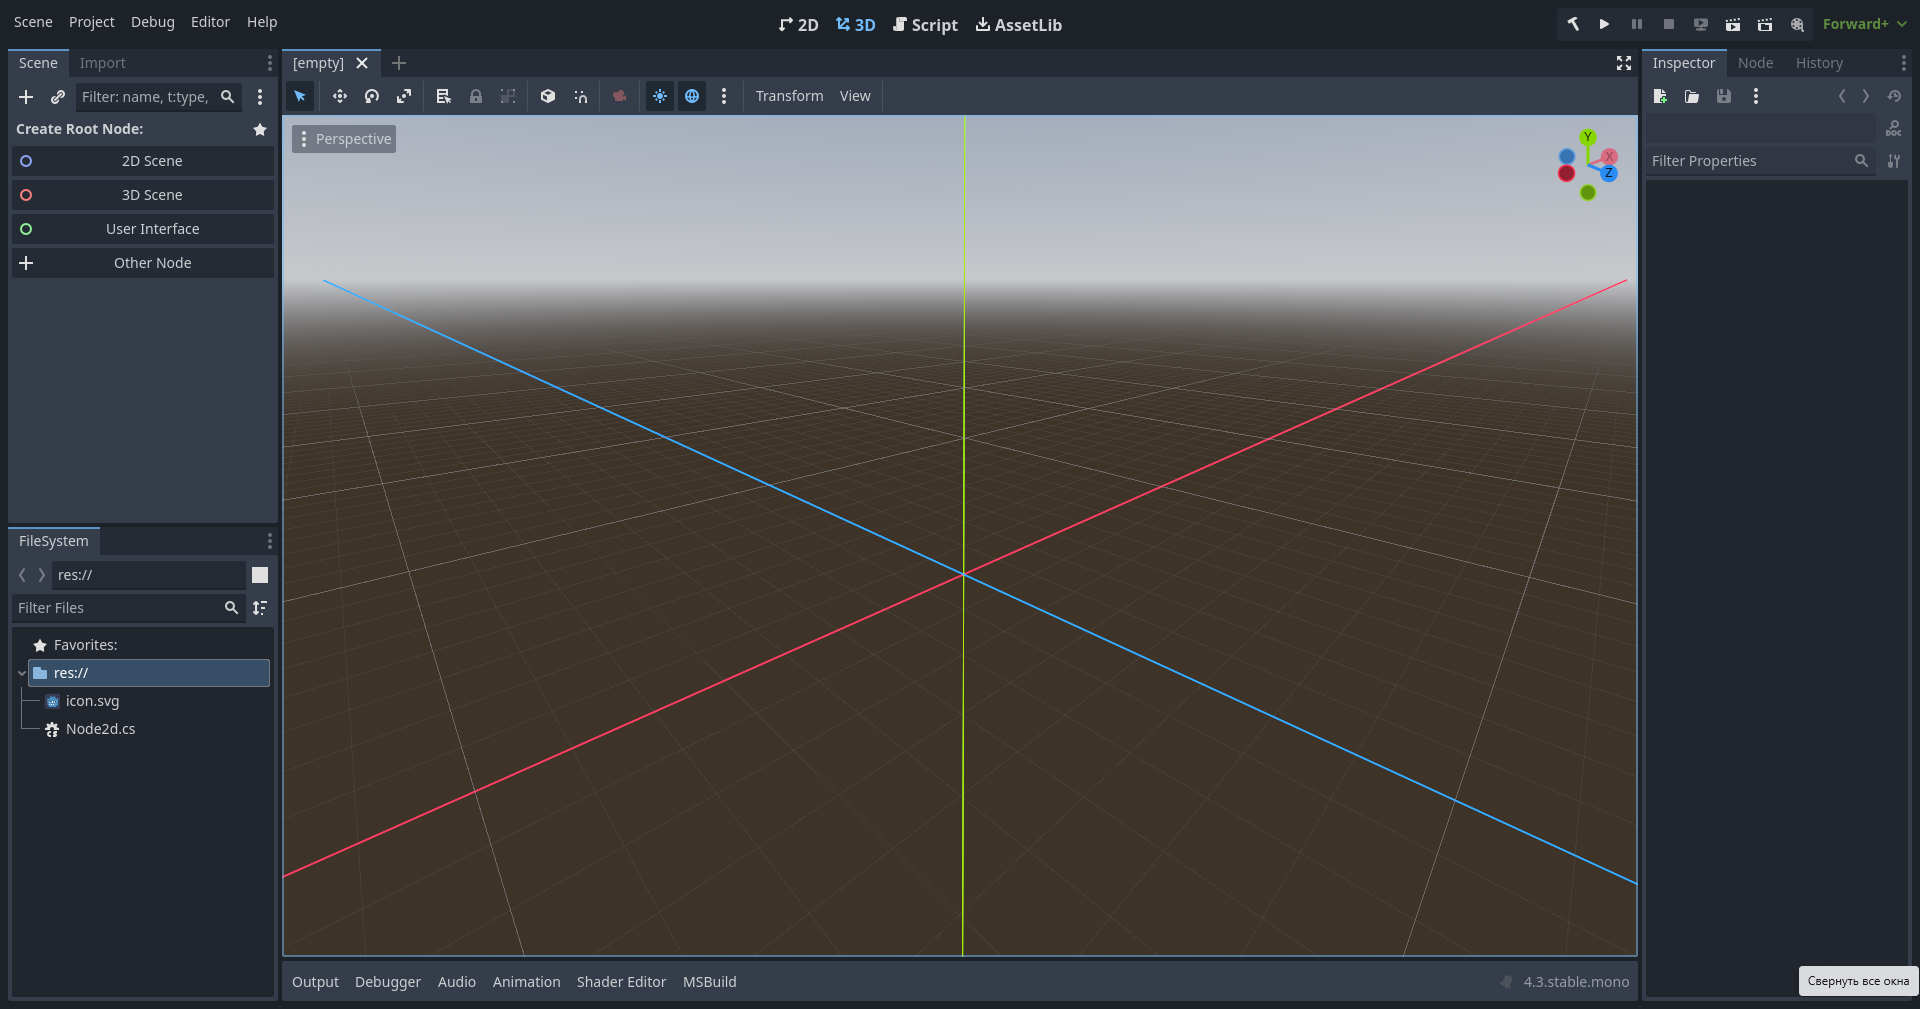
\includegraphics[width=\textwidth]{pictures/godot-editor.png}
            \caption{Редактор Godot}\label{ris2.1}
        \end{figure}
        При запуске и создании проекта нас встречает редактор с пустой 3D-сценой (Рисунок \ref{ris2.1}). Для начала разработки необходим проект C\#, который автоматически создается при подключении любого C\#-скрипта к любому узлу. Была создана новая 2D-сцена и корневой узел, к которому затем привязан скрипт. В папке проекта автоматически создадутся .csproj и .sln файлы, с которыми уже можно работать в Visual Studio. Поскольку клиент является одним из модулей, вся директория клиента будет являться частью большего по масштабу проекта, в который также включены следующие проекты, которые были разработаны в рамках курсовой работы:

        \begin{itemize}
            \item Server -- модуль основного процесса, отвечающего за инициализацию остальных модулей проекта;
            \item SharedObjects -- библиотека классов, содержащая объекты, которые присутствуют в других модулях. Например, класс Gamestate нужен и серверу, и клиенту, чтобы обмениваться информацией об игровом состоянии. Также в этом проекте реализован игровой цикл;
            \item VoiceRecognitionModule -- модуль ASR. В нем находится Vosk -- библиотека для распознавания речи. Цикл этого модуля заключается в том, что он непрерывно считывает голосовой потока с клиента и преобразует его в текст, после чего он пытается интерпретировать команду и отправить ее серверу;
            \item VoiceResponseModule -- модуль TTS, который, на каждый запрос о выполненной команде, синтезирует аудиоответ игроку и отправляет его на клиент.
        \end{itemize}

        Эти модули были написаны на версии .NET 8.0, в то время как C\# проект Godot имеет целевую ОС .NET 6.0, из-за чего возникают проблемы при сборке проекта. Если поменять целевую ОС, то сборка проходит успешно.

        Далее нужно подключить отладчик Visual Studio к проекту Godot. Для этого надо создать новый параметр запуска и указать путь для движка.
        
        После всех настроек структура решения изображена на рисунке в \textbf{приложении В}.

        Структура проекта на Citrus, в свою очередь, изображена на рисунке в \textbf{приложении Г}.

        Очевидно преимущество структуры C\#-проекта на Godot, так как она позволяет легко находить нужные файлы и быстро ориентироваться в проекте. Citrus же имеет сложную и громоздкую структуру, которая затрудняет навигацию по проекту. Большинство этих файлов не имеют практического смысла для разработчика, они лишь представляют собой низкоуровневый код и нужны для функционирования движка. 

        В последнюю очередь, стоит определиться со структурой Godot-проекта для комфортной навигации по редактору:
        \begin{itemize}
            \item Assets -- директория с ассетами игр, такими как спрайты, шрифты, звуки и т.д.;
            \item Scenes -- сцены игры. Сцены в Godot -- это отдельные файлы, которые могут содержать узла, скрипты и другие ресурсы. Каждая сцена может быть загружена и использована в игре;
            \item Scripts -- директория со скриптами, содержащие всю логику клиентского приложения. Для каждой сцены скрипты будут помещаться в отдельные директории, поскольку сцены друг от друга никак не зависят и общих ресурсов не имеют;
            \item Shaders -- директория с шейдерами, которые используются для создания эффектов в игре. Шейдеры -- это программы, которые выполняются на графическом процессоре и позволяют создавать визуальные эффекты, не затрагивая логику игры.
        \end{itemize}

        Подводя итог, настройка Godot 4.3 с поддержкой Mono, привязка проекта к Visual Studio 2022 и выстраивание чёткой структуры каталогов создали удобную и прозрачную основу для разработки. Унификация целевого фреймворка на .NET 6.0 позволила собрать все компоненты без конфликтов, а конфиг запуска в IDE обеспечил комфортную отладку C\#-скриптов в среде Godot. В результате проект обрел надёжную и масштабируемую архитектуру, готовую к дальнейшей разработке.


    \subsection{Разработка клиентской части}

        \subsubsection{Система сцен и узлов}
        
        Система сцен и узлов в Godot лежит в основе построения любой игровой логики и интерфейса. Вместо монолитных классов движок предлагает композицию: каждое игровое или вспомогательное звено представлено отдельным узлом (Node), а сцена (Scene) — это файл-контейнер, в котором узлы организованы в древовидную структуру.

        Узел сам по себе ничего не рисует и не обрабатывает ввод, пока не получает <<роли>> через тип. Так, Node2D отвечает за двумерное позиционирование и отрисовку спрайтов, а Control-узлы служат для построения GUI. При необходимости один и тот же узел можно добавить в разные сцены, комбинировать и расширять его функциональность скриптами на C\#.

        Сцена в Godot она может быть сохранена в файл .tscn или .scn и затем <<инстанцирована>> в качестве дочернего элемента в любой другой сцене. Это позволяет организовать вложенные уровни: главная игровая сцена содержит сцену игрового мира, а та, в свою очередь, включает узлы с игровыми объектами. Кроме того, Godot поддерживает механизм наследования сцены: на основе базового шаблона можно создать <<наследника>>, добавив или переопределив узлы и скрипты. Это удобно для быстрой генерации вариантов однородных игровых объектов или экранов меню с общим видом.

        Рабочий процесс обычно выглядит так: в редакторе создаётся корневая сцена, где располагаются узлы — камера, фон, интерфейс. Каждый узел настраивается через инспектор: задаются свойства, подключаются скрипты, выставляются приоритеты отрисовки.

        У любого узла можно переопределять методы, отвечающие за логику конкретных событий. Так, метод Ready вызывается единоразово при инициализации узла, Process -- каждый игровой кадр, а Input -- после любого пользовательского ввода. При разработке будут переопределяться именно эти три метода.

        \subsubsection{Глобальные переменные}

        Иногда для реализации игровой логики необходимо передавать информацию между сценами. Для решения этой проблемы в Godot существует концепция глобальных переменных. Глобальные переменные реализуются через механизм singletons, когда пользовательский класс подключается в настройках Godot-проекта и становится доступен из любой сцены по выбранному имени. Через такой singleton удобно хранить состояние о сетевом клиенте информацию об игроке и общие настройки, такие как IP-адрес и порт сервера. Доступ к этим переменным прост -- достаточно инициализировать объект в узле и обратиться к полю или методу класса, что избавляет от необходимости передавать данные вручную между узлами и сценами.

        \subsubsection{Сцена главного меню}

        Главное меню -- первая сцена, которая встречает игрока. Через него задаются параметры подключения к серверу и имя игрока. Для его создания используются Control-узлы, представляющие различные примитивные элементы интерфейса, такие как ярлык, поле для ввода текста, кнопка, контейнеры для организации этих элементов. Через редактор Godot элементы накладываются друг на друга, образуя иерархическую древовидную структуру.

        Для подключения к серверу и началу игрового процесса достаточно трех полей ввода -- для имени игрока, IP-адреса и порта сервера, а также кнопки, по нажатии на которую происходит переключение между сценами. У объекта Button есть событие OnButtonPressed, которое вызывается каждый раз при ее нажатии. К этому событию можно привязать метод, который будет осуществлять переключение между сценами, предварительно обновляя глобальные переменные, которые пользователь ввел в соответствующие поля ввода:

        \begin{lstlisting}[caption=Реализация логики главного меню]
public override void _Ready()
{
    IPInput = GetNode<TextEdit>("VBoxContainer/IPEdit");
    portInput = GetNode<TextEdit>("VBoxContainer/PortEdit");
    nameInput = GetNode<TextEdit>("VBoxContainer/PlayerNameEdit");

    GetNode<Button>("VBoxContainer/StartButton").Pressed += OnButtonPressed;
}
private void OnButtonPressed()
{
    string playerName = nameInput.Text;
    string ip = IPInput.Text;
    string port = portInput.Text;
    NetworkClient netClient = new NetworkClient();

    Global globals = GetNode<Global>("/root/Global");

    globals.NetworkClient = netClient;
    globals.PlayerName = playerName;
    globals.IPAddress = ip;
    globals.Port = port;
    GetNode<Button>("VBoxContainer/StartButton").Disabled = true;

    GetTree().ChangeSceneToFile("res://Scenes/tile_map.tscn");
}
        \end{lstlisting}

        \subsubsection{Основная сцена}

            В основной сцене реализована непосредственно игровая логика: взаимодействие с сервером, обработка пользовательского ввода и отрисовка игрового состояния, присылаемого сервером. В этой сцене находятся следующие узлы:

            \textbf{RootNode}

            RootNode -- корневой узел сцены. Сам по себе не содержит какой-либо игровой логики и не является элементом интерфейса. Данный узел служит связующим звеном между его потомками. 
            
            \textbf{TileMapLayer}

            TileMapLayer представляет собой расширение встроенного в Godot типа узла TileMap, отвечающее за отрисовку и управление одним <<слоем>> тайловой карты. Каждый экземпляр TileMapLayer хранит ссылку на ресурс TileSet, в котором каждому ID тайла сопоставлен спрайт, область коллизий и дополнительные свойства. При инициализации уровня из серверных данных TileMapLayer для каждой клетки вызывает метод SetCell, размещая нужный тайл на сетке с указанным Z-индексом. Отдельные слои (например, база, объекты и подсветка выбранных клеток) создаются как несколько TileMapLayer с разными Z-индексами, что позволяет менять любой слой в реальном времени без перерисовки остальных.

            TileMapLayer поддерживает разные формы тайлов -- квадратную, шестиугольную, изометрическую и квадратную со сдвигом, что существенно облегчит разработку, так как не придется реализовывать игровое поле самостоятельно, как было при разработке игры на Citrus.

            Для клиента было реализовано четыре узла TileMapLayer -- слои с рамками клеток, фоном (белый -- свободная клетка, зеленый -- союзный юнит, красный -- вражеский), иконку юнита, а также слой из серых тайлов -- <<туман войны>>

            Для того чтобы создать тайл на слое, нужно подготовить набор текстур, который называется TileSet. В Godot можно быстро создать набор тайлов, загрузив изображение (Рисунок \ref{ris2.4}):
            \begin{figure}[H]
                \centering
                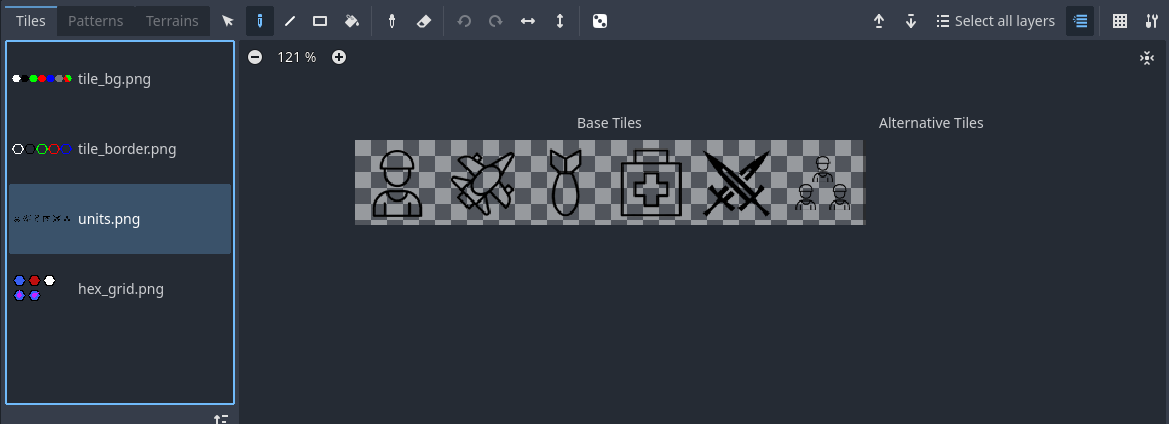
\includegraphics[width=\textwidth]{pictures/godot_tileset.png}
                \caption{Наборы тайлов для слоев TileMapLayer}\label{ris2.4}
            \end{figure}

            При наложении друг на друга, слои образуют понятное для игрока игроков поле, визуализирующее игровое состояние.

            \textbf{CursorHover}

            \textit{CursorHover} -- это узел примитивного типа, к которому привязан скрипт с логикой наведения курсора на TileMapLayer, чтобы отображать ту клетку, на которую в текущий момент наведен курсор. Это нужно в первую очередь для удобства навигации игрока по игровой карте. Это реализовывается через смену тайла на слое BorderTileLayer, который отвечает за рамку шестиугольной клетки.

            При реализации было учтено несколько важных нюансов: при захвате положения курсора возвращаются координаты относительно окна приложения. То есть, если камера будет находиться не в нулевых координатах, то будет выбран не тот тайл, на который наведен курсор. То же самое касается и приближения камеры.

            Для решения этой проблемы нужно учитывать эти параметры камеры при вычислении нужного тайла.

            \begin{lstlisting}[caption=Реализация подсветки тайла]
public override void _Process(double delta)
{
    Viewport viewport = GetViewport();
    Vector2 mousePos = viewport.GetMousePosition();
    mousePos -= viewport.GetWindow().Size / 2; //adjust position by window size
    mousePos /= camera.Zoom; //adjust position by camera zoom
    mousePos += camera.Position; //adjust position by camera coords
    Vector2I tilePos = borderLayer.LocalToMap(mousePos);

    var data = borderLayer.GetCellTileData(tilePos);

    if (data == null)
        return;

    if (currentTile == null || tilePos != currentTile)
    {
        if (currentTile != null && borderLayer.GetCellAtlasCoords(currentTile.Value)[0] != 4)
        {
            OnMouseExitedTile(currentTile.Value);
        }
        currentTile = tilePos;
        if (data != null && borderLayer.GetCellAtlasCoords(tilePos)[0] != 4)
            OnMouseEnteredTile(tilePos);
    }
}

private void OnMouseEnteredTile(Vector2I tileCoords)
{
    borderLayer.SetCell(tileCoords, 1, new Vector2I(2, 0));
}

private void OnMouseExitedTile(Vector2I tileCoords)
{
    borderLayer.SetCell(tileCoords, 1, new Vector2I(1, 0));
}
            \end{lstlisting}


            \textbf{VoiceReceiverNode}

            VoiceReceiverNode -- узел, в котором происходит обработка ввода пользователем звука с микрофона, и в отдельном потоке воспроизводится аудиоответы от сервера. При нажатии на пробел создается канал gRPC и начинается запись голосовой команды. После того как игрок отпускает клавишу, запись останавливается и отправляется в модуль TTS.
            \begin{lstlisting}[caption=Цикл обработки голосового ввода]
public void Update(double delta)
{
    bool isSpacePressed = Input.IsKeyPressed(Key.Space);
    if (_wasSpacePressed && !isSpacePressed)
    {
        waveInEvent.StopRecording();
        Thread.Sleep(100);
        channel?.Dispose();
        callForSendVoice?.Dispose();
        channel = null;
        voiceStreamingClient = null;
        callForSendVoice = null;
    }

    if (!_wasSpacePressed && isSpacePressed)
    {
        channel ??= GrpcChannel.ForAddress("http://localhost:12344");
        voiceStreamingClient ??= new SpeechToCommand.SpeechToCommandClient(channel);
        callForSendVoice ??= voiceStreamingClient.AudioToText();
        waveInEvent.StartRecording();
    }

    _wasSpacePressed = isSpacePressed;
}
            \end{lstlisting}
            
            \textbf{Camera2D}

            Без камеры навигация по игровому полю будет невозможна: его площадь в разы превышает размер окна, и игрок будет видеть лишь малую его долю. Для ее реализации Godot предоставляет узел Camera2D, и разработчику лишь остается запрограммировать ее поведение.

            Примитивным вариантом было бы реализовать перемещение камеры при помощи клавиатуры, но в контексте стратегии в реальном времени это весьма неудобно. В играх такого жанра навигация по игровой карте традиционно осуществляется при помощи компьютерной мыши. В данном случае будет реализовано перемещение камеры при удерживании правой кнопки мыши; при отпускании камера будет фиксировать положение. После того как игрок нажал на кнопку, фиксируются старые координаты камеры и положение курсора, и пока игрок не отпустит ее, каждый кадр камера будет смещаться на разницу между текущим и зафиксированным положением курсора, тем самым обеспечивая плавное перемещение.

            Также имеет смысл реализовать приближение и отдаление камеры, поскольку карта может быть произвольных масштабов, и для быстрой навигации может быть необходимо отдалить камеру.

            Стоит учесть, что, как и в случае с узлом CursorHover, координаты курсора также возвращаются относительно окна. Эта проблема решается аналогичным образом.

            \begin{lstlisting}[caption=Реализация перемещения камеры]
public override void _Input(InputEvent @event)
{
    Viewport viewport = GetViewport();
    Vector2 mousePos = viewport.GetMousePosition();
    mousePos -= viewport.GetWindow().Size / 2; //adjust position by window size
    mousePos += currentCamCoords; //adjust position by camera coords

    if (@event is InputEventMouseButton ev && ev.ButtonIndex == MouseButton.Right)
    {
        if (ev.Pressed)
        {
            dragging = true;
            lastMousePos = mousePos;
        }
        else
        {
            currentCamCoords = Position;
            dragging = false;
        }
    }


    if (@event is InputEventMouseMotion mv && dragging)
    {
        var evPos = mv.Position;
        evPos -= viewport.GetWindow().Size / 2;
        evPos += currentCamCoords;

        var delta = evPos - lastMousePos;
        lastMousePos = evPos;
        Position -= delta/Zoom;
    }

}
            \end{lstlisting}

            \textbf{ClientNode}

            ClientNode -- основной узел сцены, в котором реализован игровой цикл. В нем происходит взаимодействие с сервером и отрисовывается игровое состояние. Перед отрисовкой кадра с сервера приходит обновленное состояние. На его основе размещаются тайлы в узлах типа TileMapLayer, причем все клетки на поле перекрываются <<туманом войны>>. После размещения юнитов поле очищается от тумана: происходит итерация по всем юнитам игрока, и для каждого юнита очищаются клетки в его радиусе обзора.
            
            В этом же узле реализована логика <<активной клетки>>: при нажатии левой кнопки мыши на клетку, она помечается как активная, и в верхнем левом углу отображается список юнитов, находящихся в ней, который обновляется динамически. Чтобы достигнуть этого, составляется актуальный список юнитов, присланный от сервера, затем происходит итерация по дочерним узлам элемента интерфейса, отвечающего за отображение юнитов на клетке. Если оказывается, что в окне находится юнит, которого нет в актуальном списке, то этот элемент удаляется. Если оказывается, что кого-то не хватает, создается новый элемент и инициализируется. Важно проводить итерацию от последнего дочернего к первому, чтобы в случае удаления не нарушалась индексация.
            
        
        \subsubsection{Heads-Up Display (HUD)}

            Одно из преимуществ Godot -- обильное количество встроенных инструментов для верстки сложных элементов пользовательского интерфейса. HUD вынесен в отдельный CanvasLayer, что обеспечивает его отрисовку всегда поверх игровой сцены и независимость от движения камеры. Внутри CanvasLayer строится древовидная структура Control-узлов. Были реализованы следующие элементы интерфейса:

            \textbf{CoordsWindow}

            Небольшое окно в левом нижнем углу экрана, отображающее координаты клетки, на которую наведен курсор. Это нужно для удобства навигации и отдачи голосовых команд игроком. Данные обновляются на узле CursorHover: перед подсветкой наведенного курсором узла, вызывается метод UpdateCoordsHUD.
            \begin{lstlisting}[caption=обновление интерфейса]
void UpdateHUD(Vector2I coords)
{
    Label xLabel = coordsBox.GetChild<Label>(0);
    Label yLabel = coordsBox.GetChild<Label>(1);

    xLabel.Text = $"X: {coords[0]}";
    yLabel.Text = $"Y: {coords[1]}";
}
            \end{lstlisting}

            \textbf{CellInfoBase и CellInfoContainer}
            
            В процессе игры необходимо знать не только координаты определенной клетки, но и информацию о юнитах, которые на ней находятся. Для этого был создан шаблон панели с информацией о юните. Корневым узлом шаблона является PanelContainer -- контейнер с настраиваемым задним фоном (Рисунок \ref{ris2.5}). На него помещены узлы типа VBoxContainer и HBoxContainer для корректного размещения узлов, несущих в себе информацию о юните.

            Из информативных узлов присутствуют ярлыки для позывного юнита и значению здоровья в текстовом виде, TextureRect -- область, в которой отрисовывается текстура; в ней будет присутствовать иконка юнита. Наконец, для визуального отображения оставшегося здоровья был добавлен TextureProgressBar -- полоса прогресса, на которую можно добавить текстуру. Узел этого типа имеет поле Range, в котором можно настраивать <<полноту>> текстуры в виде процентного значения.

            Также в целях отладки была добавлена кнопка типа TextureButton для отдачи команды юнитам в обход голосовому интерфейсу.
            

            \begin{figure}[H]
                \centering
                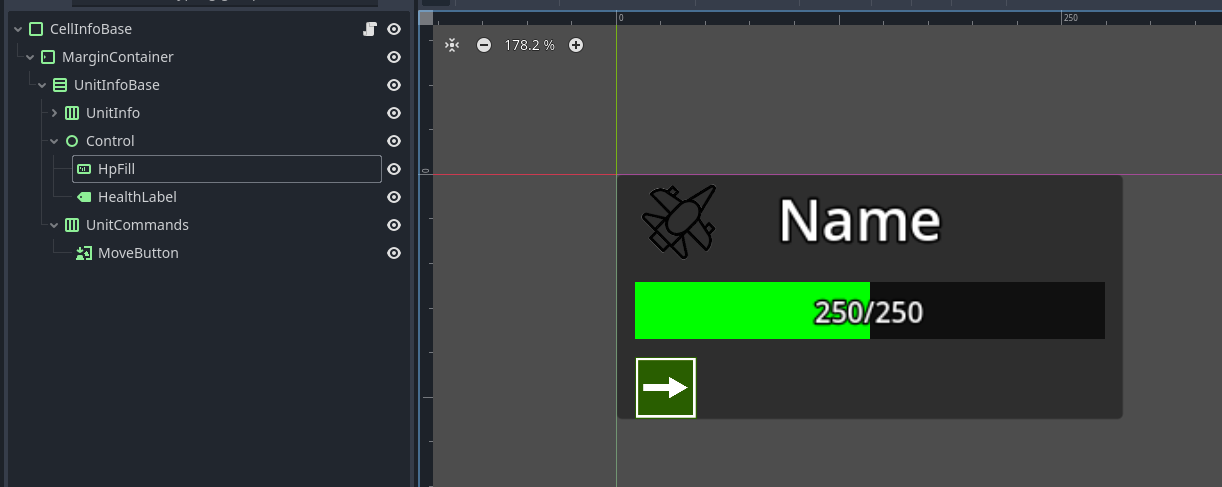
\includegraphics[width=\textwidth]{pictures/cellinfobase.png}
                \caption{Шаблон элемента CellInfo}\label{ris2.5}
            \end{figure}

            Поскольку это шаблон для одного из множества юнитов на поле боя, этот элемент интерфейса нужно сохранить в отдельную сцену, чтобы программно создавать его для каждого юнита. Когда на выделенной клетке есть какой-то юнит, происходит <<инстанциация>> сцены, что создает новый узел, повторяющий всю структуру сцены. Этот узел в последствии прикрепляется в специальный контейнер с возможностью прокрутки содержимого, становясь его наследником.
            \begin{lstlisting}[caption=Создание экземпляра шаблона]
var unitInfoScene = GD.Load<PackedScene>("res://Scenes/cell_info_base.tscn");
CellInfoBase panel = unitInfoScene.Instantiate<CellInfoBase>();
panel.Setup(selectedCell.Value, currentUnit.Health, currentUnit.MaxHealth, unitId, atlCoords, currentUnit.Nickname);

panel.Handler = (bool toggledOn) =>
{
    OnMoveButtonPressed(panel, toggledOn);
};
panel.MoveButton.Toggled += panel.Handler;

cellInfo.AddChild(panel);
            \end{lstlisting}


    \subsection{Доработка серверной части}

        После завершения разработки клиентской части необходимо было доработать серверную часть. На момент сдачи курсовой работы серверная часть обладала базовым функционалом для работы сетевой составляющей, игрового цикла и голосового интерфейса.

        Для демонстрации возможностей клиента на Godot были добавлены новые геймплейные возможности и устранены недочеты.

        \subsubsection{Единственный юнит на клетке}
        Одним из недочетов было то, что игровое поле было запрограммировано таким образом, что на одной клетке в один момент времени мог находиться лишь один юнит. Когда на нее переходил другой юнит, пока она была занята, информация о расположении этого юнита на клетке пропадала, в то время как сам юнит оставался в игровом состоянии.

        Игровая клетка представляет из себя объект HexCell, являющегося частью объекта HexGrid. В нем было поле CellUnitId -- уникальный идентификатор юнита в игровом мире. Метод UpdateCellUnit заменял значение этой переменной, что приводило к противоречиям в игровом состоянии -- у клетки был один идентификатор юнита, а у того, которого сместили -- координаты клетки сместившего его юнита.

        Эта проблема была решена, заменив поле типа int на список уникальных идентификаторов. Для корректной работы также были обновлены методы UpdateCellUnit и RemoveCellUnit, которые добавляли и удаляли элемент из списка соответственно.

        \subsubsection{Ошибка в изменении коллекции при итерации}

        При перемещении юнитов сервер периодически завершал работу с ошибкой, которая указывала на изменение коллекции при итерации, в следствие чего происходило обращение по несуществующему индексу. Оказалось, что во время сериализации игрового состояния оно успевало обновиться, из-за чего при сериализации списков их размер оказыватся некорректен.

        Решением проблемы была блокировка ресурсов во время итерации с помощью ключевого слова lock. Таким образом, если объект оказывался <<занят>>, другая часть кода, запрашивавшая доступ к этому же ресурсу, ждала освобождение объекта.

        \subsubsection{Сражение юнитов}

        Ключевая механика любой RTS -- сражение на поле боя. До начала работы была лишь реализована механика передвижения. Для задания минимальной играбельности необходимо было реализовать сражение хотя бы на базовом уровне.

        Поскольку теперь на одной клетке могут находится несколько юнитов разных игроков, сражения будет обрабатывать HexCell. Далее описан один игровой цикл сражения. 
        
        Составляются списки юнитов каждого игрока, затем происходит итерация по этим двум спискам: если юнит может атаковать, он атакует первого попавшегося врага и уходит на перезарядку. Если не может, то счетчик перезарядки увеличивается на время, которое прошло с момента прошлого игрового цикла. Если прошло достаточно времени, юнит атакует по той же логике. Если какой-либо из юнитов погибает, их идентификаторы записываются в отдельный массив. После атаки погибшие юниты удаляются из игры. Сражение продолжается, пока на клетке не останутся юниты, принадлежащие к одной команде.

        Реализация сражения юнитов продемонстрирована в листинге в \textbf{приложении Д}.
    \subsection{Итог главы}

    В практической части были последовательно решены поставленные задачи. Сначала было настроено окружение разработки (Godot 4.3+Mono, Visual Studio 2022), определена чёткую структуру решения с отдельными проектами Server, SharedObjects, VoiceRecognitionModule и VoiceResponseModule и привязало всё это к единому .sln-решению.

    Далее в клиенте на Godot были реализованы следующие и узлы: главного меню на Control-контейнерах и глобальных переменных, слои TileMapLayer, реализующие игровое поле, CursorHover для подсветки клеток, гибкую камеру с управлением мышью и клавиатурной навигацией, VoiceReceiverNode для голосовых команд и ClientNode, который по обновлённому состоянию от сервера расставляет тайлы, очищает <<туман войны>>, реагирует на клики и обновляет HUD через CanvasLayer и сигналы.
    
    На сервере было усовершенствовано представление клеток, устранен Race Condition при сериализации состояния, а также реализован базовый цикл сражения внутри HexCell.
    
    В результате практической части получился минимально жизнеспособный прототип сетевой RTS: кроссплатформенный клиент на Godot+C\#, голосовой интерфейс на Vosk+gRPC, авторитетный сервер с логикой юнит-менеджмента и боёв, а также удобный UI-слой для отображения ресурсов, статусов и выбранных клеток. Эта архитектура заложила прочную основу для дальнейшего расширения игровых механик и обогащения голосового опыта.
    \pagebreak
    
    % !TEX root =..\main.tex
\section*{ЗАКЛЮЧЕНИЕ}\addcontentsline{toc}{section}{ЗАКЛЮЧЕНИЕ}

В результате выполненной работы получился полнофункциональный прототип сетевой RTS-игры, готовый к дальнейшей доработке и расширению. В отличие от 
первоначальной реализации на движке Citrus, где разработка упиралась в органичения движка, такие как отсутствие кроссплатформенности, 
слабую документацию и фрагментарный набор готовых инструментов, Godot позволил получить кроссплатформенный клиент со значительно расширенным функционалом 
благодаря его гибкой системе сцен и узлов, интуитивному редактору и встроенной поддержке C\#. Серверная часть сохраняет роль авторитетного хоста, обеспечивая
синхронность игровых состояний, а голосовой интерфейс на основе Vosk и gRPC работает стабильно и независимо от внешних облачных сервисов.

Godot доказал свою пригодность как для опытных, так и для начинающих разработчиков: понятные принципы композиции сцен и мгновенная <<горячая>> перезагрузка 
скриптов сокращают время обучения и позволяют сосредоточиться непосредственно на геймплейных механиках. 
Активное сообщество и подробная документация дают возможность быстро найти решение практически любой технической задачи, а визуальные инструменты для 
верстки HUD, настройки камер и работы с тайл-картами делают создание интерфейсов приятным и наглядным.

В будущем прототип легко может быть масштабирован: предусмотрены механизмы добавления новых типов юнитов, расширения правил боя, интеграции нейросетевых 
TTS-модулей и более сложных сценариев сетевого взаимодействия. Полученный результат может служить базой для учебных проектов, демо-версий коммерческих 
продуктов или открытого сообщества разработчиков. Благодаря открытому исходному коду и модульной архитектуре эта работа заложила надёжную платформу 
для любых дальнейших экспериментов и развития.
    \pagebreak

    % !TEX root =..\main.tex
\section*{СПИСОК ИСПОЛЬЗОВАННЫХ ИСТОЧНИКОВ}\addcontentsline{toc}{section}{СПИСОК ИСПОЛЬЗОВАННЫХ ИСТОЧНИКОВ}
\begin{enumerate}[label=\arabic*)]
    \item Bradfield C. Godot 4 Game Development Projects. -- Packt Publishing, 2023.
    \item Citrus API Documentation. [Электронный ресурс] -- URL: https://game-forest.github.io/Citrus/api/Lime.html
    \item Godot Engine 4.3 documentation in English. [Электронный ресурс] -- URL: https://docs.godotengine.org/en/4.3
    \item C\# language documentation. [Электронный ресурс] -- URL: https://learn.microsoft.com/en-us/dotnet/csharp
    \item gRPC C\# Guide -- Official Documentation. [Электронный ресурс] -- URL: https://grpc.io/docs/languages/csharp
    \item Болотаев Р.А. Godot Generals. [Электронный ресурс] -- URL: https://github.com/Olimp666/GodotGenerals
\end{enumerate}
    \pagebreak

    % !TEX root =..\main.tex
\appendix
\section*{ПРИЛОЖЕНИЯ}\addcontentsline{toc}{section}{ПРИЛОЖЕНИЕ А}
\setcounter{section}{1}
\setcounter{figure}{0}
\setcounter{table}{0}
\setcounter{lstlisting}{0}
\renewcommand{\thefigure}{}
\renewcommand{\thetable}{}
\renewcommand{\thelstlisting}{}


\captionsetup[table]{labelformat=empty, labelsep=none, justification=centering, position=top,font=fourteenpt}
\captionsetup[lstlisting]{labelformat=empty, labelsep=none, justification=centering, position=top,font=fourteenpt}
\captionsetup[figure]{labelformat=empty, labelsep=none, justification=centering, position=top,font=fourteenpt}

\section*{ПРИЛОЖЕНИЕ А}
\begin{figure}[H]
    \centering
    \caption{Файловая структура C\#-проекта на Godot}\label{app1}
    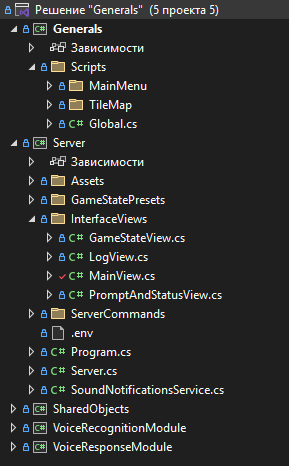
\includegraphics[height=0.75\textheight]{pictures/godot_fs.png}
\end{figure}
\pagebreak

\section*{ПРИЛОЖЕНИЕ Б}
\begin{figure}[H]
    \centering
    \caption{Файловая структура C\#-проекта на Citrus}\label{app2}
    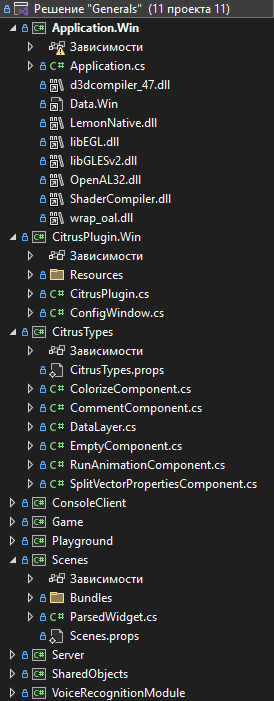
\includegraphics[height=0.85\textheight]{pictures/citrus_fs.png}
\end{figure}
\pagebreak

\section*{ПРИЛОЖЕНИЕ В}
\begin{lstlisting}[caption=Цикл сражения юнитов]
    public void ProcessFight(GameState gs, TimeSpan timeDelta)
    {
        lock (_lock)
        {
            List<BaseUnit> p1Units = [];
            List<BaseUnit> p2Units = [];
            List<int> deadUnitsIds = [];
            foreach (int unitId in CellUnitIds)
            {
                var curUnit = gs.GetUnitById(unitId);
                if (curUnit.PlayerId == 0)
                    p1Units.Add(curUnit);
                else
                    p2Units.Add(curUnit);
            }
            AttackEnemies(p1Units, p2Units, deadUnitsIds, timeDelta);
            foreach (var deadId in deadUnitsIds)
            {
                RemoveCellUnit(deadId);
                gs.RemoveUnit(deadId);
            }
        }
    }
    private void AttackEnemies(List<BaseUnit> allies, List<BaseUnit> enemies, List<int> dead, TimeSpan timeDelta)
    {
        int p = 0;
        for (int i = 0; p < enemies.Count && i < allies.Count; i++)
        {
            var curUnit = allies[i];
            var curEnemy = enemies[p];
            if (curUnit.OnCooldown)
            {
                curUnit.Elapsed += timeDelta;
                if (curUnit.Elapsed >= TimeSpan.FromSeconds(curUnit.AttackSpeed))
                {
                    curUnit.Elapsed = TimeSpan.Zero;
                    curUnit.OnCooldown = false;
                }
            }
            else
            {
                curEnemy.Health -= curUnit.AttackDamage;
                curUnit.OnCooldown = true;
            }
    
            if (curEnemy.Health <= 0)
            {
                dead.Add(curEnemy.UnitId);
                p++;
            }
        }
    }
\end{lstlisting}\label{app4}
\pagebreak

\section*{ПРИЛОЖЕНИЕ Г}
\begin{table}[ht]
    \caption{Список голосовых команд}
    \centering
    \renewcommand{\arraystretch}{1.2}
    \renewcommand{\tablename}{Табл.}
    \begin{tabularx}{\textwidth}{|X|X|}
    \hline
    \textbf{Команда}&\textbf{Описание}\\
    \hline
    Перемещение&Игрок называет позывной юнита, говорит слово <<перемещение>>, затем называет координаты нужной клетки, после чего названный юнит идет в указанную клетку. Если у юнита нет возможности перемещаться, команда игнорируется.\\
    \hline
    Бомбардировка&Игок называет позывной юнита класса <<артиллерия>>, говорит слово <<бомбардировка>>, называет координаты, и в результате все юниты в указанной клетке и в клетках по соседству получают урон.\\
    \hline
    \end{tabularx}
\end{table}
\pagebreak

\section*{ПРИЛОЖЕНИЕ Д}
\begin{table}[ht]
    \caption{Сравнение TTS решений}
    \centering
    \begingroup
    \fontsize{10}{12}\selectfont
    \renewcommand{\arraystretch}{1.2}
    \renewcommand{\tablename}{Табл.}
    \resizebox{\textwidth}{!}{
    \begin{tabularx}{\textwidth}{|X|X|X|X|X|X|X|X|}
    \hline
    \textbf{Решение}&\textbf{Качество голоса}&\textbf{Задержка, мс}&\textbf{Зависимо-сти}&\textbf{C\#-SDK}&\textbf{Офлайн}&\textbf{Платфор-мы}&\textbf{Стоимость}\\
    \hline
    Speech-Synthesizer&низкое (монотонно)&50–100&.NET Framework на Windows&\textbf{встроен-ный}&\textbf{да}&Windows&\textbf{бесплатно}\\
    \hline
    Google Cloud TTS&высокое (естественно)&~200–300&стабильный интернет&есть&нет&кросс-платфор-менно&платно, по минутам\\
    \hline
    Azure Speech&высокое (естественно)&~200–300&стабильный интернет&есть&нет&кросс-платфор-менно&платно, по минутам\\
    \hline
    Yandex SpeechKit&высокое (естественно)&~150–200&табильный интернет&есть&нет&кросс-платфор-менно&платно, по минутам\\
    \hline
    Coqui TTS&среднее–высокое&CPU: ~200–300, GPU: <100&Python/модели, GPU (рекомендуется)&нет&да&кросс-платфор-менно&бесплатно\\
    \hline
    \end{tabularx}
    }
    \endgroup
\end{table}

    \pagebreak
\end{document}